\documentclass{beamer}
\mode<presentation>
\usetheme{CambridgeUS}
\usepackage[russian]{babel}
\usepackage[utf8]{inputenc}
\usepackage[T2A]{fontenc}
\usepackage{sansmathaccent}

\usepackage{verbatim}
\usepackage{alltt}

\pdfmapfile{+sansmathaccent.map}
\title[GIT]{Системы управления версиями. GIT}
\author{Наумов Д.А., доц. каф. КТ}
\date[18.04.2019] {Основы компьютерных наук, 2019}

\begin{document}

%ТИТУЛЬНЫЙ СЛАЙД
\begin{frame}
  \titlepage
\end{frame}
  
%СОДЕРЖАНИЕ ЛЕКЦИИ
\begin{frame}
  \frametitle{Содержание лекции}
  \tableofcontents  
\end{frame}
  
%РАЗДЕЛ 1
\section{Управление версиями}

\begin{frame}{Введение}
\begin{block}{Система управления версиями}
система, сохраняющая изменения в одном или нескольких файлах так, чтобы потом можно было восстановить определённые старые версии.
\end{block}
Задачи, решаемые СУВ:
\begin{itemize}
\item вернуть файлы к прежнему виду;
\item вернуть к прежнему состоянию весь проект;
\item сравнить изменения с какого-то времени;
\item увидеть, кто последним изменял модуль, который дал сбой, кто создал проблему;
\item восстановить проект в любом состоянии.
\end{itemize}
\end{frame} 

\begin{frame}
\begin{block}{Система управления версиями}
\begin{center}
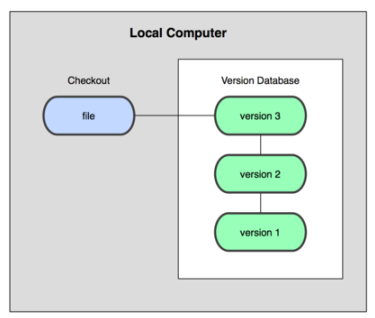
\includegraphics[scale=0.5]{images/local.png}
\end{center}
\end{block}
Особенность локальных СУВ:
\begin{itemize}
\item имеется база данных, в которой хранятся все изменения нужных файлов;
\item базы данных хранится на локальном компьютере;
\item изменения хранятся в виде набора патчей между парой изменений;
\end{itemize}
Пример: утилита \textit{rcs}.
\end{frame} 

\begin{frame}
Цель: ЦСУВ - сотрудничество удаленных разработчиков.
\begin{block}{Централизованная система управления версиями}
\begin{center}
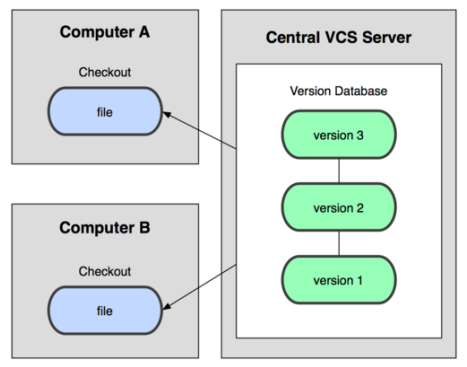
\includegraphics[scale=0.4]{images/central.png}
\end{center}
\end{block}
Особенность ЦСУВ:
\begin{itemize}
\item все отслеживаемые файлы хранятся на сервере;
\item клиенты получают копии файлов с сервера;
\end{itemize}
Пример: \textit{CSV}, \textit{Subversion}, \textit{Perforce}.
\begin{itemize}
\item + контроль за разработчиками; проще администрирование;
\item - взаимодействие без сервера невозможно; потеря истории при повреждении цетральной БД;
\end{itemize}
\end{frame} 

\begin{frame}{Хранение изменений файлов в ЦСУВ}
\begin{block}{Данные хранятся как изменения к базовой версии для каждого файла}
\begin{center}
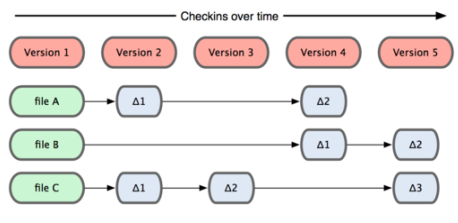
\includegraphics[scale=0.7]{images/patch.png}
\end{center}
\end{block}
Хранимыме данные - набор файлов и изменений, сделанных для каждого из этих файлов во времени.
\end{frame} 

\begin{frame}
\begin{block}{Распределенная система управления версиями}
\begin{center}
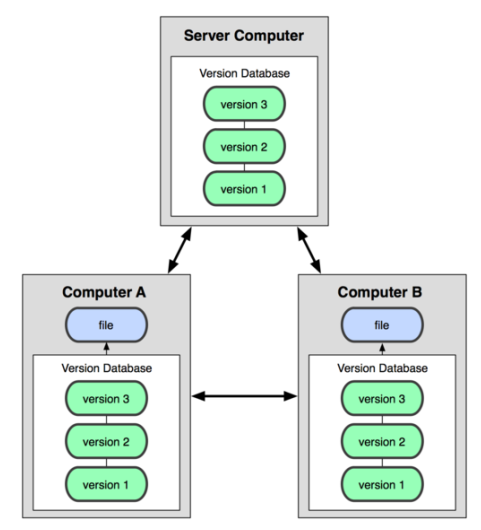
\includegraphics[scale=0.3]{images/decentral.png}
\end{center}
\end{block}
Особенность РСУВ:
\begin{itemize}
\item клиенты полностью копируют репозиторий;
\item клиентский репозиторий может быть скопирован обратно на сервер, чтобы восстановить БД;
\item есть возможность работать с несколькими удаленными репозиториями; 
\end{itemize}
Пример: \textit{Git}, \textit{Mercurial}, \textit{Bazaar}, \textit{Darcs}.
\end{frame} 

\begin{frame}{Хранение изменений файлов в РСУВ}
\begin{block}{Данные хранятся как слепки состояния проекта}
\begin{center}
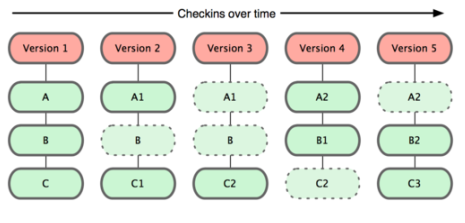
\includegraphics[scale=0.7]{images/checking.png}
\end{center}
\end{block}
Хранимыме данные - наборо слепков состояния файловой системы.
\end{frame} 

\section{Операции в GIT}
\begin{frame}{Операции в GIT}
Для большинства операций не нужно соединение с сетью:
\begin{itemize}
\item просмотр истории проекта;
\item просмотр различий версий файла (например, сейчас и месяц назад);
\item возможность сохранения изменений в БД
\end{itemize}
Контроль целостности данных:
\begin{itemize}
\item вычисление контрольных сумм SHA-1;
\item невозможно "незаметно" изменить файл или каталог;
\end{itemize}
\begin{center}

\includegraphics[scale=0.5]{images/sha.png}
\end{center}
Данные в системы только добавляются. Сложно заставить GIT удалить данные или сделать что-то неотменяемое.
\end{frame} 

\begin{frame}{Состояние файлов в GIT}
В Git файлы могут находиться в одном из трёх состояний:
\begin{itemize}
\item зафиксированном - файлы уже сохранёны в локальной базе;
\item изменённом - файлы, которые поменялись, но ещё не были зафиксированы;
\item подготовленном - изменённые файлы, отмеченные для включения в следующий коммит.
\end{itemize}
Стандартный рабочий процесс:
\begin{center}
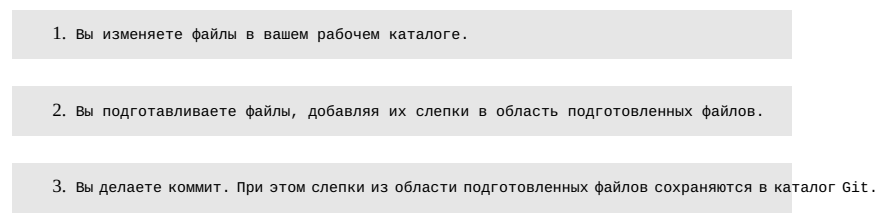
\includegraphics[scale=0.5]{images/process.png}
\end{center}
\end{frame} 

\begin{frame}
Три части проекта с использованием GIT:
\begin{itemize}
\item каталог Git — место, где Git хранит метаданные и базу данных объектов проекта;
\item рабочий каталог — это извлечённая из базы копия определённой версии проекта;
\item область подготовленных файлов — файл, хранящийся в каталоге Git, содержащий информацию о том, что должно войти в следующий коммит.
\end{itemize}
\begin{center}
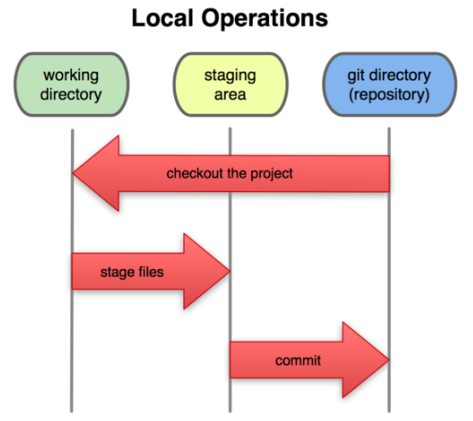
\includegraphics[scale=0.4]{images/catalog.png}
\end{center}
\end{frame} 

\begin{frame}
\begin{block}{Установка GIT}
\begin{itemize}
\item в Linux (Debian): \textit{apt-get install git-core}
\item в Windows: \textit{http://code.google.com/p/msysgit}
\item в Mac: \textit{http://code.google.com/p/git-osx-installer}
\end{itemize}
\end{block}
\begin{block}{Настройка GIT: git config}
\begin{itemize}
\item файл /etc/gitconfig содержит значения, общие для всех пользователей вашей системы
и всех их репозиториев (--system);
\item Файл ~/.gitconfig хранит настройки конкретного пользователя (--global);
\item конфигурационный файл в каталоге Git (.git/config) в том репозитории, где вы
находитесь в данный момент 
\end{itemize}
\end{block}
\end{frame} 

\begin{frame}
\begin{block}{Настройка пользователя}
\begin{center}
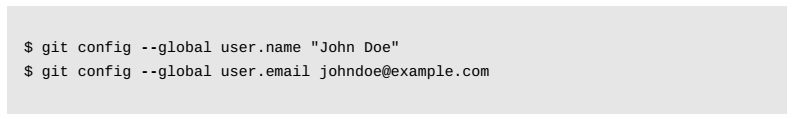
\includegraphics[scale=0.55]{images/username.png}
\end{center}
\end{block}
\begin{block}{Настройка редактрока}
\begin{center}
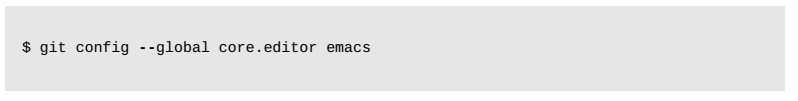
\includegraphics[scale=0.55]{images/editor.png}
\end{center}
\end{block}
\begin{block}{Настройка утилиты сравнения}
\begin{center}
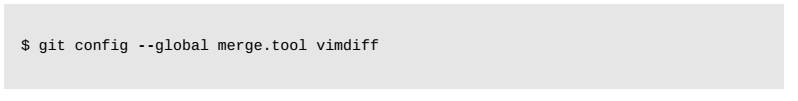
\includegraphics[scale=0.55]{images/diff.png}
\end{center}
\end{block}
\end{frame}

\begin{frame}
\begin{block}{Просмотр настроек}
\begin{center}
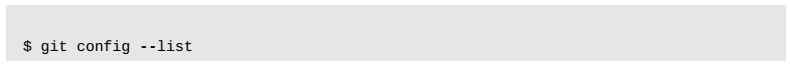
\includegraphics[scale=0.55]{images/config-1.png}
\end{center}
\end{block}
\begin{center}
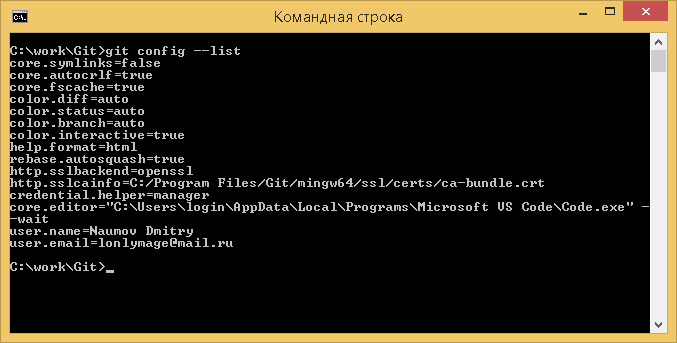
\includegraphics[scale=0.55]{images/config-2.png}
\end{center}
\end{frame}

\begin{frame}
\begin{block}{Получение помощи}
\begin{center}
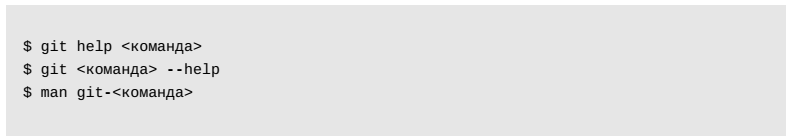
\includegraphics[scale=0.55]{images/help-1.png}
\end{center}
\end{block}
\begin{block}{Получение помощи по конкретной команде}
\begin{center}
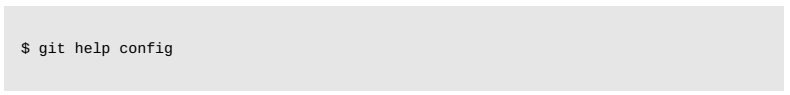
\includegraphics[scale=0.55]{images/help-2.png}
\end{center}
\end{block}
\end{frame}

\section{Основы работы в GIT}
\begin{frame}{Создание репозитория Git}
\begin{block}{Новый репозиторий в текущем каталоге}
\begin{center}
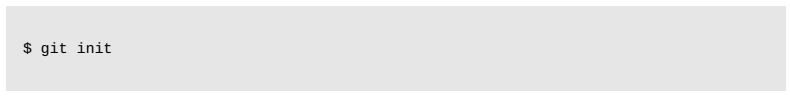
\includegraphics[scale=0.55]{images/init-1.png}
\end{center}
\begin{center}
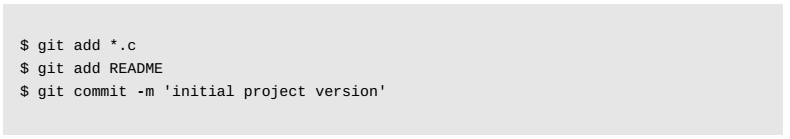
\includegraphics[scale=0.55]{images/init-2.png}
\end{center}
\end{block}
\begin{block}{Клонирование существующего репозитория}
\begin{center}
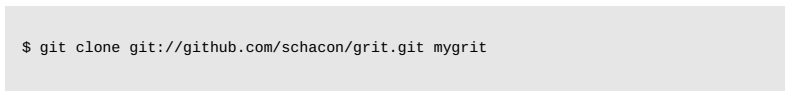
\includegraphics[scale=0.55]{images/init-3.png}
\end{center}
\end{block}
\end{frame}

\begin{frame}{Запись изменений в репозиторий}
Файлы в рабочем каталоге могут быть в состоянии:
\begin{itemize}
\item отслеживаемые - под версионным контролем (неизмененные, измененные, подготовленными к коммиту).
\item неотслеживаемые - любые файлы, которые не входили в последний слепок состояния и не подготовлены к коммиту. 
\end{itemize}
\begin{block}{Жизненный цикл состояния файлов проекта}
\begin{center}
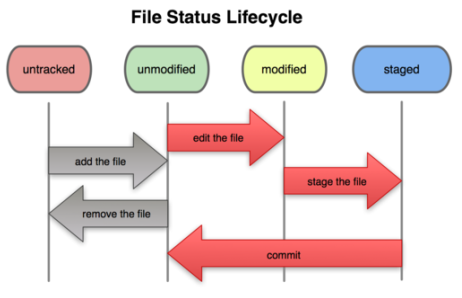
\includegraphics[scale=0.5]{images/lifecycle.png}
\end{center}
\end{block}
\end{frame}

\begin{frame}{Определение состояний файлов}
\begin{block}{git status}
\begin{center}
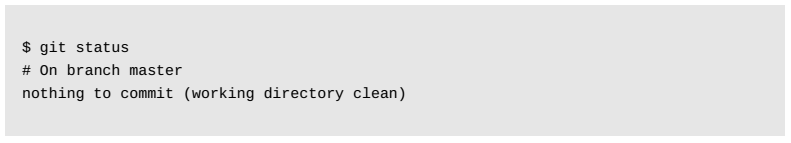
\includegraphics[scale=0.5]{images/git-status-1.png}
\end{center}
\end{block}
\begin{block}{git status после создания нового файла}
\begin{center}
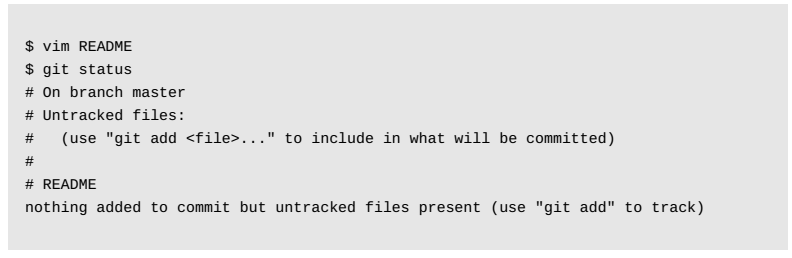
\includegraphics[scale=0.5]{images/git-status-2.png}
\end{center}
\end{block}
\end{frame}

\begin{frame}{Отслеживание новых файлов}
\begin{block}{git add}
\begin{center}
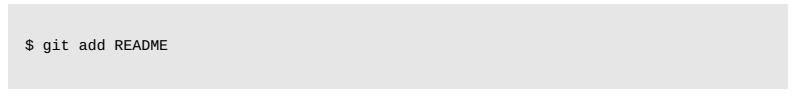
\includegraphics[scale=0.5]{images/git-add-1.png}
\end{center}
\end{block}
\begin{block}{git status после добавления отслеживания}
\begin{center}
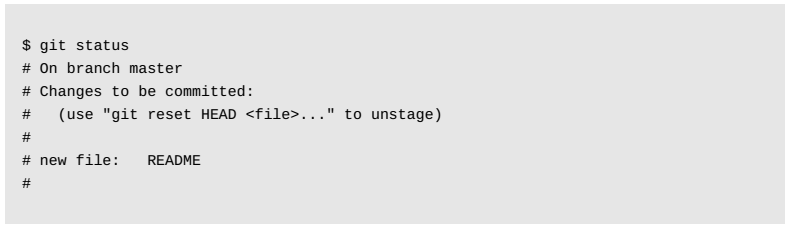
\includegraphics[scale=0.5]{images/git-add-2.png}
\end{center}
\end{block}
\end{frame}

\begin{frame}{Индексация отслеживаемых файлов}
\begin{block}{изменим benchmarks.rb, потом - git status}
\begin{center}
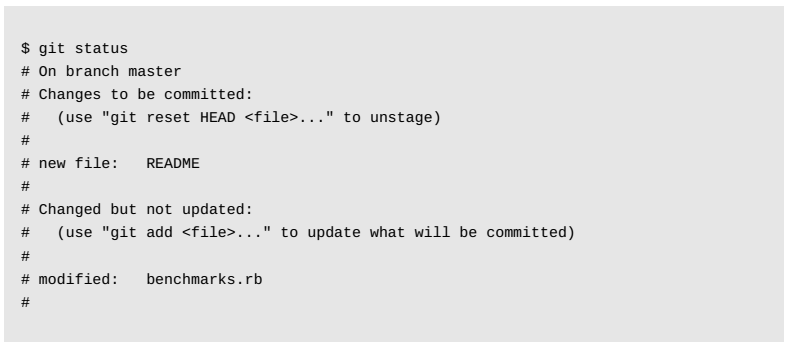
\includegraphics[scale=0.5]{images/git-index-1.png}
\end{center}
\end{block}
«Changed but not updated» — отслеживаемый файл был изменен в рабочем каталоге, но пока не проиндексирован. 
\end{frame}

\begin{frame}{Индексация отслеживаемых файлов}
\begin{block}{git add, потом - git status}
\begin{center}
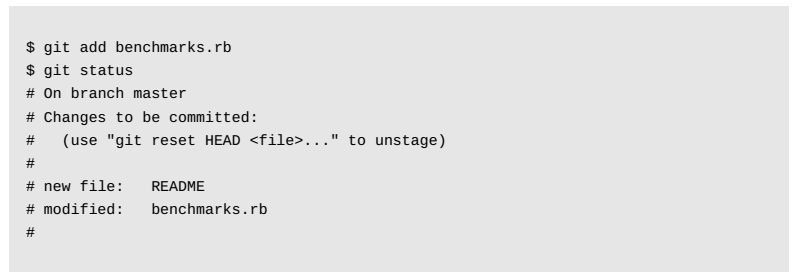
\includegraphics[scale=0.5]{images/git-index-2.png}
\end{center}
\end{block}
Оба файла проиндексированы и войдут в следующий коммит. 
\end{frame}

\begin{frame}{Индексация отслеживаемых файлов}
\begin{block}{снова изменим файл и проверим - git status}
\begin{center}
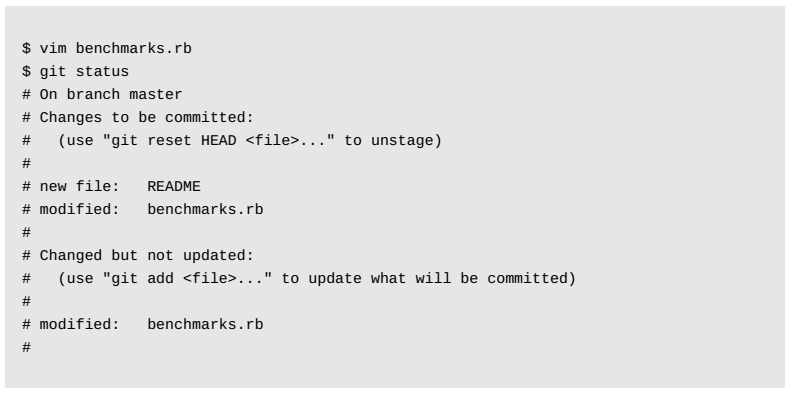
\includegraphics[scale=0.5]{images/git-index-3.png}
\end{center}
\end{block}
benchmarks.rb - проиндексированный и непроиндексированный одновременно.
\end{frame}

\begin{frame}{Игнорирование файлов}
\begin{block}{Файл .gitignore}
\begin{center}
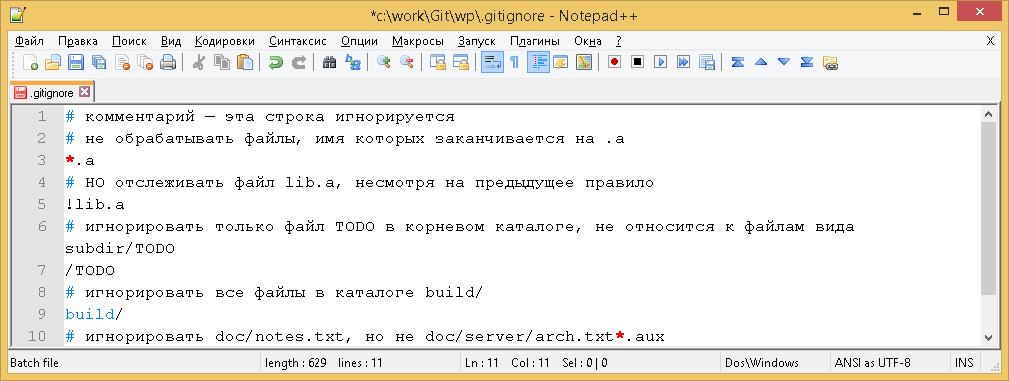
\includegraphics[scale=0.3]{images/gitignore-2.png}
\end{center}
\end{block}
Glob-шаблоны (упрощенные регулярные выражения:
\begin{itemize}
\item $*$ - соответствует 0 или более символам; 
\item $[abc]$ — соответствует любому cимволу из указанных в скобках  (в данном случае a,b,c);
\item $?$ - соответствует одному символу; 
\item $[0-9]$ - соответствует любому символу из интервала (в данном случае от 0 до 9).
\end{itemize}
\end{frame}

\begin{frame}{Просмотр различий в файлах}
Команда \textit{git diff} сравнивает содержимое вашего рабочего каталога с содержимым индекса.
Результат показывает еще не проиндексированные изменения.
\begin{block}{git diff}
\begin{center}
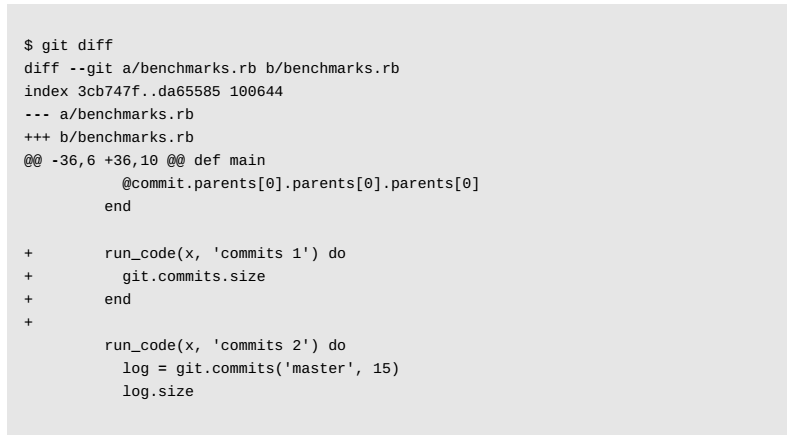
\includegraphics[scale=0.4]{images/diff-1.png}
\end{center}
\end{block}
\end{frame}

\begin{frame}{Фиксация изменений}
\begin{block}{git commit}
\begin{center}
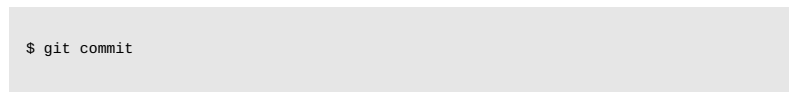
\includegraphics[scale=0.5]{images/commit.png}
\end{center}
\end{block}
Эта команда откроет выбранный текстовый редактор:
\begin{center}
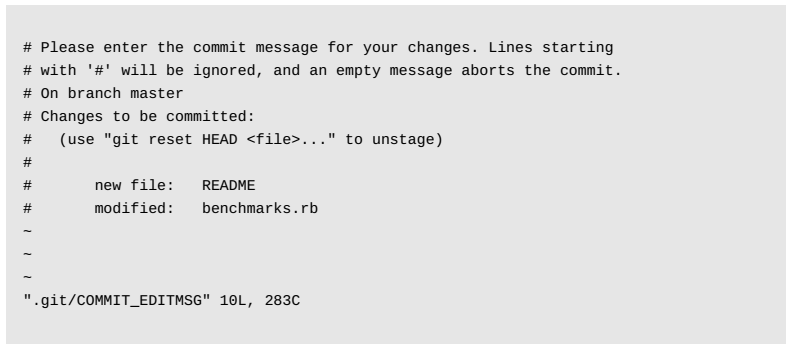
\includegraphics[scale=0.5]{images/commit-1.png}
\end{center} 
\end{frame}

\begin{frame}{Фиксация изменений}
\begin{block}{git commit -m текст сообщения}
\begin{center}
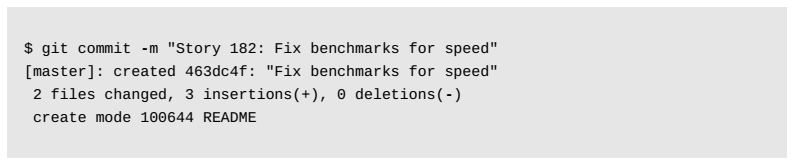
\includegraphics[scale=0.5]{images/commit-2.png}
\end{center}
Коммит вывел информацию:
\begin{itemize}
\item на какую ветку вы выполнили коммит (master);
\item какая контрольная сумма SHA-1 у этого коммита (463dc4f);
\item сколько файлов было изменено;
\item статистику по добавленным/удаленным строкам в этом коммите.
\end{itemize}
\end{block}
\end{frame}

\begin{frame}{Игнорирование индексации}
\begin{block}{git commit -a -m текст сообщения}
\begin{center}
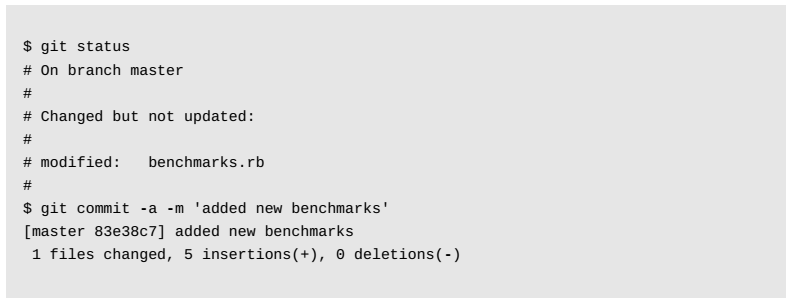
\includegraphics[scale=0.5]{images/commit-3.png}
\end{center}
\end{block}
\end{frame}

\begin{frame}{Удаление файла}
Для того чтобы удалить файл из Git, необходимо удалить его из отслеживаемых файлов (точнее, удалить его из индекса), а затем выполнить коммит. 
\begin{block}{git rm имяфайла}
\begin{center}
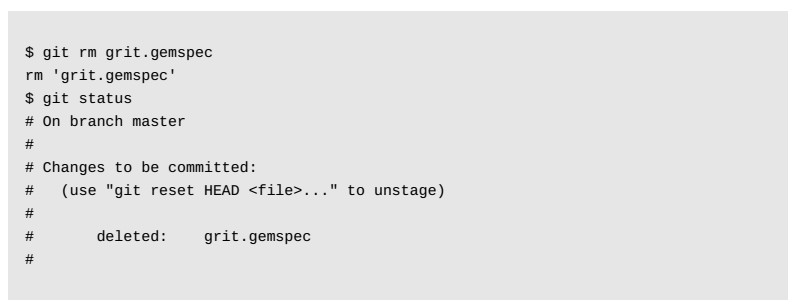
\includegraphics[scale=0.5]{images/rm-2.png}
\end{center}
\end{block}
Если просто удалить файл из рабочего каталога, он будет показан в секции
«Changed but not updated».
\end{frame}

\begin{frame}{Удаление файла}
\begin{block}{git rm --cached имяфайла}
\begin{center}
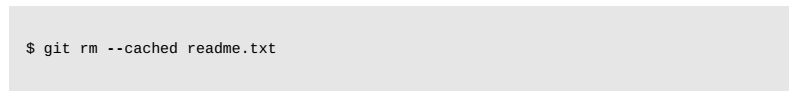
\includegraphics[scale=0.5]{images/rm-3.png}
\end{center}
\end{block}
\begin{block}{использование шаблонов}
\begin{center}
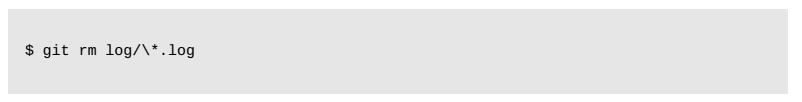
\includegraphics[scale=0.5]{images/rm-4.png}
\end{center}
\begin{center}
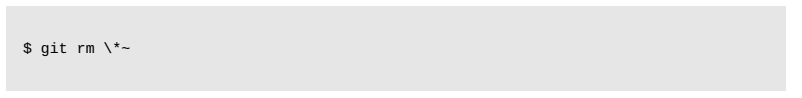
\includegraphics[scale=0.5]{images/rm-5.png}
\end{center}
\end{block}
\end{frame}

\begin{frame}{Перемещение файла}
\begin{block}{git mv}
\begin{center}
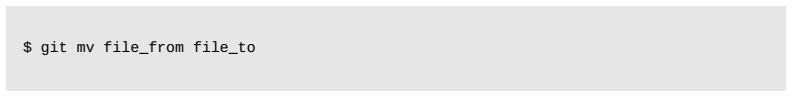
\includegraphics[scale=0.5]{images/mv-1.png}
\end{center}
\end{block}
\begin{block}{результат перемещения}
\begin{center}
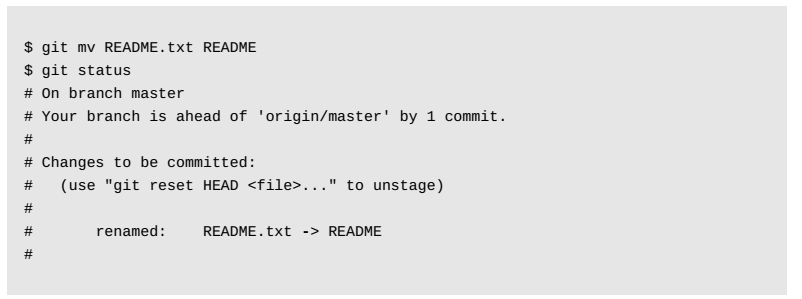
\includegraphics[scale=0.5]{images/mv-2.png}
\end{center}
\end{block}
\end{frame}

\begin{frame}{Просмотр истории коммитов}
\begin{block}{git log}
\begin{center}
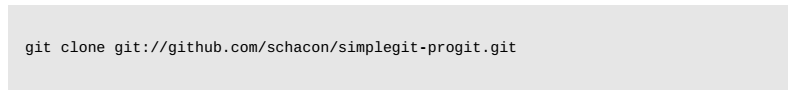
\includegraphics[scale=0.5]{images/log-1.png}
\end{center}
\end{block}
\begin{block}{результат выполнения команды}
\begin{center}
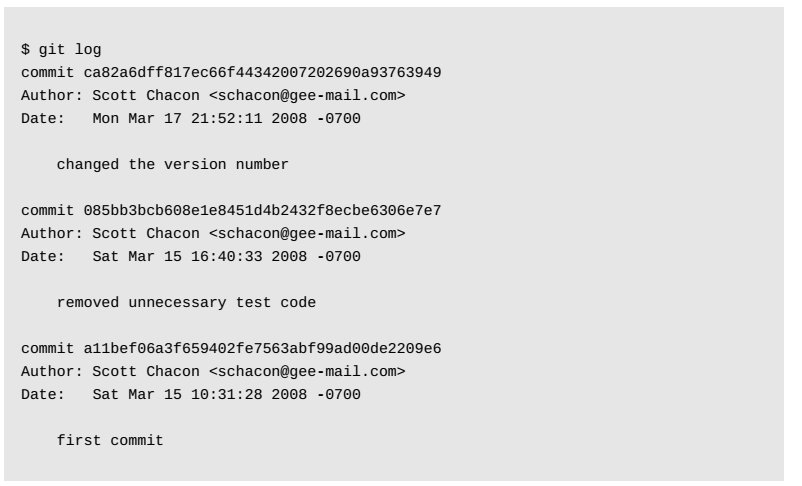
\includegraphics[scale=0.5]{images/log-2.png}
\end{center}
\end{block}
\end{frame}

\begin{frame}{Отмена последнего коммита}
\begin{block}{git commit --amend}
\begin{center}
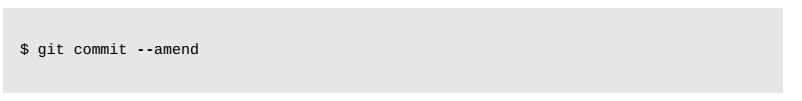
\includegraphics[scale=0.5]{images/ammed-1.png}
\end{center}
\end{block}
\begin{block}{второй коммит заменяет результаты первого}
\begin{center}
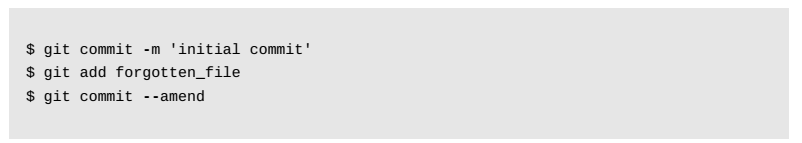
\includegraphics[scale=0.5]{images/ammed-2.png}
\end{center}
\end{block}
\end{frame}

\begin{frame}{Отмена индексации файла}
\begin{block}{git reset HEAD file}
\begin{center}
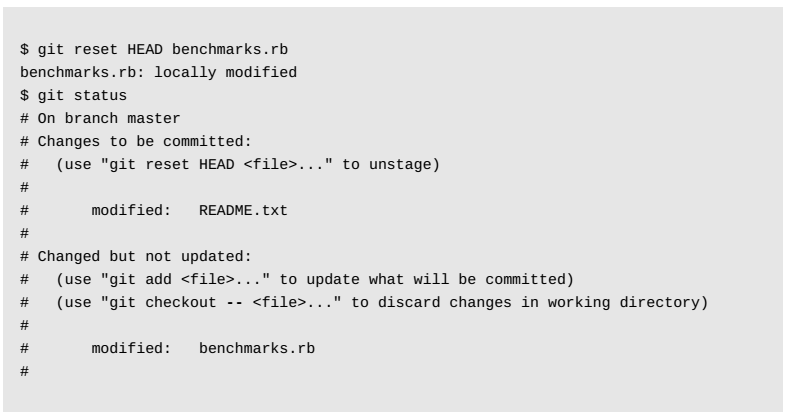
\includegraphics[scale=0.5]{images/reset.png}
\end{center}
\end{block}
Отмена изменения файла: git checkout -- benchmarks.rb
\end{frame}

\section{Работа с удаленными репозиториями}
\begin{frame}{Работа с удаленными репозиториями}
\begin{block}{Удаленный репозиторий}
модификации проекта, которые хранятся в интернете или ещё где-то в сети.
\end{block}
Совместная работа включает в себя управление удалёнными репозиториями и помещение
(push) и получение (pull) данных в и из них тогда, когда нужно обменяться результатами работы.
Управление удалёнными репозиториями включает:
\begin{itemize}
\item умение добавлять удалённые репозитории;
\item умение удалять те из них, которые больше не действуют;
\item умение управлять различными удалёнными ветками;
\item умение определять их отслеживание. 
\end{itemize}
\end{frame}

\begin{frame}{Отображение удаленных репозиториев}
\begin{block}{git remote}
\begin{center}
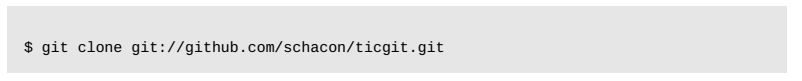
\includegraphics[scale=0.5]{images/remote-1.png}
\end{center}
\begin{center}
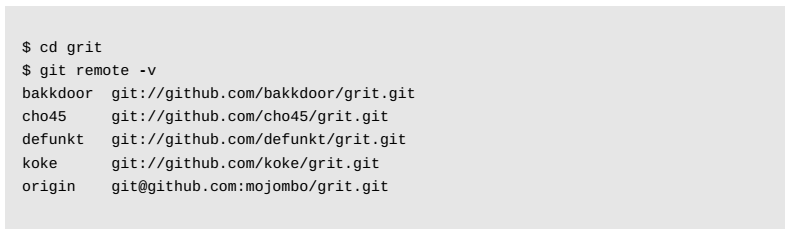
\includegraphics[scale=0.5]{images/remote-2.png}
\end{center}
\end{block}
\end{frame}

\begin{frame}{Добавление удаленных репозиториев}
Добавить новый удалённый Git-репозиторий под именем-сокращением \textit{git remote add}:
\begin{center}
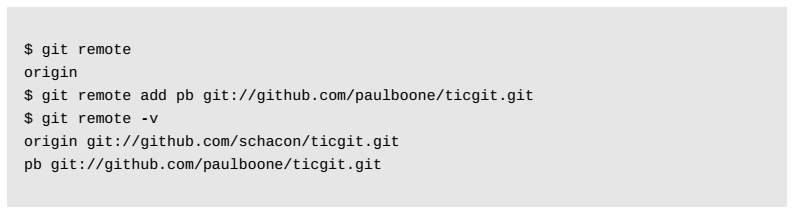
\includegraphics[scale=0.4]{images/remote-3.png}
\end{center}
Теперь вы можете использовать в командной строке имя pb вместо полного URL. 
\begin{center}
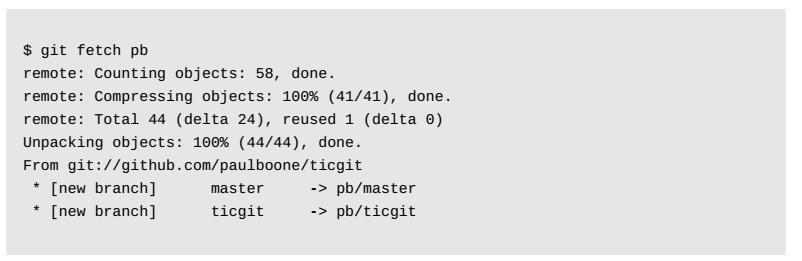
\includegraphics[scale=0.4]{images/remote-4.png}
\end{center}
\end{frame}

\begin{frame}{fetch}
Получение данных из удаленного репозитория:
\begin{center}
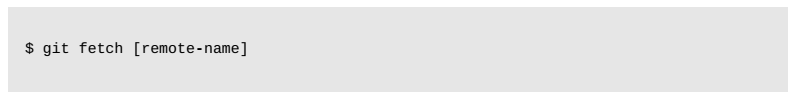
\includegraphics[scale=0.4]{images/fetch.png}
\end{center}
Данная команда:
\begin{itemize}
\item связывается с указанным удалённым проектом;
\item забирает все те данные проекта, которых у вас ещё нет;
\item в рабочем каталоге появятся ссылки на все ветки из удалённого проекта.
\end{itemize}
Команда fetch забирает данные в ваш локальный репозиторий, но не сливает их с какими-либо вашими наработками и не модифицирует то, над чем вы работаете в данный момент. Вам необходимо вручную слить эти данные с вашими, когда вы будете готовы.
\end{frame}

\begin{frame}{pull}
\textit{git pull} - получение данных из удаленного репозитория:
\begin{itemize}
\item извлекает (fetch) данные с сервера;
\item автоматически пытается слить (merge) их с кодом, над которым вы в данный момент работаете.
\end{itemize}
\end{frame}

\begin{frame}{push}
Когда вы хотите поделиться своими наработками, вам необходимо отправить (push) их в главный репозиторий. 

Команда для этого действия простая: git push [удал. сервер] [ветка].
\begin{center}
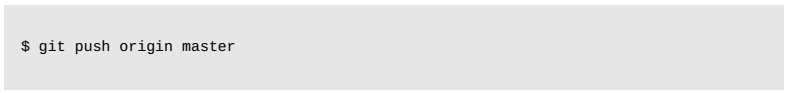
\includegraphics[scale=0.4]{images/push.png}
\end{center}
Эта команда срабатывает только в случае, если вы клонировали с сервера, на котором у
вас есть права на запись, и если никто другой с тех пор не выполнял команду push. 

Если вы и кто-то ещё одновременно клонируете, затем он выполняет команду push, а затем команду push
выполняете вы, то ваш push точно будет отклонён. 

Вам придётся сначала вытянуть (pull) их
изменения и объединить с вашими. Только после этого вам будет позволено выполнить push.
\end{frame}

\section{Ветвление в Git}
\begin{frame}{Ветвление в Git}
\begin{block}{Ветвление }
означает, что вы отклоняетесь от основной линии разработки и продолжаете работу, не вмешиваясь в
основную линию. 
\end{block}
Когда вы фиксируете изменения в Git, Git сохраняет фиксируемый объект, который содержит:
\begin{itemize}
\item указатель на снимок содержимого индекса;
\item метаданные автора и комментария;
\item ноль или больше указателей на коммиты, которые были прямыми предками этого коммита (ноль предков для
первого коммита, один — для обычного коммита и несколько — для коммита, полученного в
результате слияния двух или более веток).
\end{itemize}
\end{frame}

\begin{frame}{Пример}
Есть каталог, содержащий три файла, они индексируются и делаете коммит. 
\begin{center}
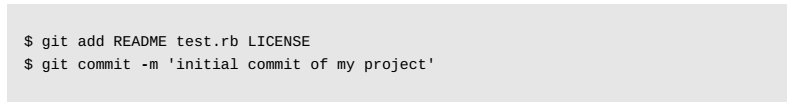
\includegraphics[scale=0.5]{images/branch-01.png}
\end{center}
При подготовке файлов для каждого из них вычисляется контрольная сумма (SHA-1), затем эти версии файлов сохраняются в Git-репозиторий, а их контрольные суммы добавляются в индекс.

При создании коммита Git:
\begin{itemize}
\item вычисляет контрольную сумму каждого подкаталога;
\item сохраняет объекты для этого дерева в Git-репозиторий;
\item создаёт объект для коммита, который имеет метаданные и указатель на корень проектного дерева. 
\end{itemize}
\end{frame}

\begin{frame}{Пример}
Данные репозитория с единственным коммитом для трех объектов. 
\begin{center}
\includegraphics[scale=0.7]{images/branch-02.png}
\end{center}
\end{frame}

\begin{frame}{Пример}
Данные объектов Git в случае нескольких коммитов. 
\begin{center}
\includegraphics[scale=0.7]{images/branch-03.png}
\end{center}
\end{frame}

\begin{frame}{Ветка в Git}
\begin{block}{Ветка}
легковесный подвижный указатель на один из этих коммитов.
\end{block}
Имя ветки по умолчанию в Git — master. При каждом новом коммите указатель сдвигается вперёд автоматически.
\begin{center}
\includegraphics[scale=0.7]{images/branch-04.png}
\end{center}
\end{frame}

\begin{frame}{Создание ветки}
\begin{block}{Создание ветки testing}
\begin{center}
\includegraphics[scale=0.5]{images/branch-05.png}
\end{center}
\end{block}
\begin{block}{Несколько веток, указывающих на историю коммитов}
\begin{center}
\includegraphics[scale=0.6]{images/branch-06.png}
\end{center}
\end{block}
\end{frame}

\begin{frame}{Указатель на текущую ветку}
Git хранит специальный указатель, который называется HEAD (верхушка) - указатель на локальную ветку, на которой вы находитесь. 
\begin{block}{Файл HEAD указывает на текущую ветку}
\begin{center}
\includegraphics[scale=0.6]{images/branch-07.png}
\end{center}
\end{block}
\end{frame}

\begin{frame}{Указатель на текущую ветку}
\begin{block}{Переход на ветку testing}
\begin{center}
\includegraphics[scale=0.5]{images/branch-08.png}
\end{center}
\end{block}
\begin{block}{HEAD указывает на другую ветку}
\begin{center}
\includegraphics[scale=0.5]{images/branch-09.png}
\end{center}
\end{block}
\end{frame}

\begin{frame}
\begin{block}{Создадим еще один коммит}
\begin{center}
\includegraphics[scale=0.5]{images/branch-10.png}
\end{center}
\end{block}
\begin{block}{Ветка, на которую указывает HEAD, движется вперёд с каждым коммитом}
\begin{center}
\includegraphics[scale=0.5]{images/branch-11.png}
\end{center}
\end{block}
\end{frame}

\begin{frame}
\begin{block}{Вернемся в ветку master (git checkout master)}
\begin{center}
\includegraphics[scale=0.5]{images/branch-12.png}
\end{center}
\end{block}
\begin{block}{История с разошедшимися ветками}
\begin{center}
\includegraphics[scale=0.5]{images/branch-13.png}
\end{center}
\end{block}
\end{frame}

\section{Основы ветвления и слияния. Пример}

\begin{frame}
\begin{block}{Что нам надо делать?}
\begin{center}
\includegraphics[scale=0.5]{images/ex-01.png}
\end{center}
\end{block}
\begin{block}{... и вдруг}
\begin{center}
\includegraphics[scale=0.5]{images/ex-02.png}
\end{center}
\end{block}
\end{frame}

\begin{frame}
\begin{block}{Создаем ветку и переходим в нее}
\begin{center}
\includegraphics[scale=0.5]{images/ex-03.png}
\end{center}
\end{block}
\begin{center}
\includegraphics[scale=0.5]{images/ex-04.png}
\end{center}
\begin{block}{Новая история коммитов}
\begin{center}
\includegraphics[scale=0.5]{images/ex-05.png}
\end{center}
\end{block}
\end{frame}

\begin{frame}
\begin{block}{Сделаем пару коммитов}
\begin{center}
\includegraphics[scale=0.5]{images/ex-06.png}
\end{center}
\end{block}
\begin{block}{Ветка iss53 передвинулась вперёд во время работы}
\begin{center}
\includegraphics[scale=0.5]{images/ex-07.png}
\end{center}
\end{block}
\end{frame}

\begin{frame}
Теперь вы получаете звонок о том, что есть проблема с веб-сайтом, которую необходимо немедленно устранить. 
\begin{block}{Создадим ветку, в которой будем работать}
\begin{center}
\includegraphics[scale=0.5]{images/ex-08.png}
\end{center}
\end{block}
Итак, надо срочно исправить ошибку - создадим для этого ветку, на которой вы будете работать.
\begin{block}{Ветка для решения срочной проблемы базируется на ветке master}
\begin{center}
\includegraphics[scale=0.5]{images/ex-09.png}
\end{center}
\end{block}
\end{frame}

\begin{frame}
\begin{block}{Ветка для решения срочной проблемы базируется на ветке master}
\begin{center}
\includegraphics[scale=0.5]{images/ex-10.png}
\end{center}
\end{block}

Вы можете запустить тесты, убедиться, что решение работает, и слить (merge) изменения
назад в ветку master, чтобы включить его в продукт. Это делается с помощью команды git
merge.
\end{frame}

\begin{frame}
\begin{block}{Сливаем ветки}
\begin{center}
\includegraphics[scale=0.5]{images/ex-11.png}
\end{center}
\end{block}
\begin{block}{После слияния ветка master указывает туда же, куда и ветка hotfix}
\begin{center}
\includegraphics[scale=0.5]{images/ex-12.png}
\end{center}
\end{block}
\end{frame}

\begin{frame}
\begin{block}{Удаляем ветку hotfix, она больше не нужна}
\begin{center}
\includegraphics[scale=0.5]{images/ex-13.png}
\end{center}
\end{block}
\begin{block}{Вернемся к нашей исходной задаче}
\begin{center}
\includegraphics[scale=0.5]{images/ex-14.png}
\end{center}
\end{block}
\end{frame}

\begin{frame}
\begin{block}{Ветка iss53 может двигаться вперёд независимо}
\begin{center}
\includegraphics[scale=0.5]{images/ex-15.png}
\end{center}
\end{block}
Работа, сделанная на ветке hotfix, не включена в файлы на ветке iss53. Если вам это необходимо, вы можете выполнить слияние ветки master в ветку iss53 посредством команды git merge master.
\end{frame}

\begin{frame}
\begin{block}{Объединим master и ветку iss53}
\begin{center}
\includegraphics[scale=0.4]{images/ex-16.png}
\end{center}
\end{block}
\begin{block}{Git автоматически определяет наилучшего общего предка для слияния веток}
\begin{center}
\includegraphics[scale=0.35]{images/ex-17.png}
\end{center}
\end{block}
\end{frame}

\begin{frame}
\begin{block}{Git автоматически создает новый коммит, содержащий результаты слияния}
\begin{center}
\includegraphics[scale=0.5]{images/ex-18.png}
\end{center}
\end{block}
\begin{block}{и удаляем ненужную ветку}
\begin{center}
\includegraphics[scale=0.5]{images/ex-19.png}
\end{center}
\end{block}
\end{frame}

\section{Основы разрешения конфликтов слияния}
\begin{frame}
Если вы изменили одну и ту же часть файла по-разному в двух ветках, которые собираетесь объединить, Git не сможет сделать это чисто. Если ваше решение проблемы №53 изменяет ту же часть файла, что и hotfix, вы получите
конфликт слияния 
\begin{center}
\includegraphics[scale=0.4]{images/conf-01.png}
\end{center}
\begin{block}{проверяем статус...}
\begin{center}
\includegraphics[scale=0.4]{images/conf-02.png}
\end{center}
\end{block}
\end{frame}

\begin{frame}
Всё, что имеет отношение к конфликту слияния и что не было разрешено, отмечено как
unmerged. Git добавляет стандартные маркеры к файлам, которые имеют конфликт, так что вы
можете открыть их вручную и разрешить эти конфликты.
\begin{center}
\includegraphics[scale=0.4]{images/conf-03.png}
\end{center}
\begin{block}{вручную разрешаем конфликт...}
\begin{center}
\includegraphics[scale=0.4]{images/conf-04.png}
\end{center}
\end{block}
После того, как вы разрешили каждую из таких секций с каждым из конфликтных файлов, выполните git add для каждого конфликтного файла.
\end{frame}

\begin{frame}
Если вы хотите использовать графические инструменты для разрешения конфликтов, можете выполнить команду git mergetool, которая запустит соответствующий графический инструмент и покажет конфликтные
ситуации:
\begin{center}
\includegraphics[scale=0.4]{images/conf-05.png}
\end{center}
\begin{center}
\includegraphics[scale=0.4]{images/conf-06.png}
\end{center}
\end{frame}

\end{document}